\documentclass[10pt]{article}

\usepackage{amsmath}
\usepackage{amssymb}

\usepackage{graphicx}

\usepackage{cite}

\usepackage{color} 

\usepackage{setspace} 
%\doublespacing

\usepackage{xr} % for cross-referencing
\externaldocument{manuscript}

% Text layout
\topmargin 0.0cm
\oddsidemargin 0.5cm
\evensidemargin 0.5cm
\textwidth 16cm 
\textheight 21cm

% Bold the 'Figure #' in the caption and separate it with a period
% Captions will be left justified
\usepackage[labelfont=bf,labelsep=period,justification=raggedright]{caption}

\bibliographystyle{nar}

% Remove brackets from numbering in List of References
\makeatletter
\renewcommand{\@biblabel}[1]{\quad#1.}
\makeatother


% Leave date blank
\date{}

\pagestyle{myheadings}

\newcommand{\bsig}{{\boldsymbol\sigma}}
\newcommand{\si}{\sigma_i}
\newcommand{\sj}{\sigma_j}

\newcommand\numberthis{\addtocounter{equation}{1}\tag{\theequation}}
\newcommand{\eq}[1]{\begin{equation*}#1\end{equation*}}
\newcommand{\eqn}[1]{\begin{equation}#1\end{equation}}
\newcommand{\eqal}[1]{\begin{align*} #1 \end{align*}}
\newcommand{\eqaln}[1]{\begin{align*} \numberthis#1 \end{align*}}
\newcommand{\eqalacc}[1]{\[\left\{\begin{aligned}#1\end{aligned}\right.\]}
\newcommand{\eqalaccn}[1]{\[\left\{\numberthis \begin{aligned}#1\end{aligned}\right.\]}

\newcommand{\bra}[1]{\langle #1 |}
\newcommand{\ket}[1]{|#1\rangle}
\newcommand{\braket}[2]{\langle#1|#2\rangle}

\title{
Imogene: identification of motifs and cis-regulatory modules
underlying gene co-regulation}
\author{Herv\'e Rouault, 
Marc Santolini ,
 Fran\c{c}ois Schweisguth,
Vincent Hakim
}
\date{\today}

\begin{document}
\maketitle

\centering \textbf{\Large Supplementary Figures}
\vskip .5cm
\makeatletter
\renewcommand{\thefigure}{
S\@arabic\c@figure}
\makeatother
\setcounter{figure}{0}


\begin{figure}[!htbp]
\begin{center}
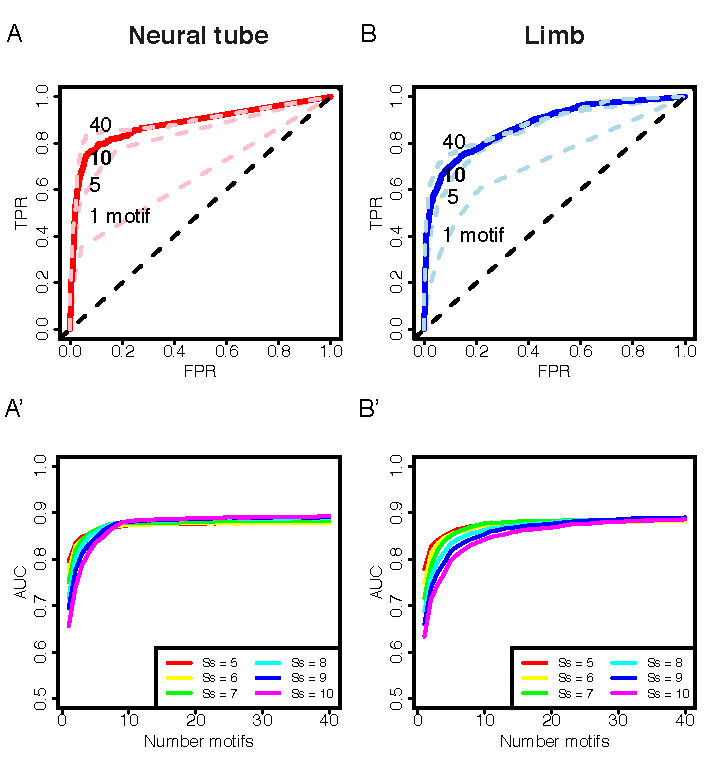
\includegraphics[width=12cm]{../figures-sub/figS1.pdf}
\end{center}
\caption{ {\bf Dependence of the predictions on the number of scoring motifs }
  ROC plots obtained at optimal scanning threshold using the Halpern-Bruno
  evolutionary model are shown for the neural tube (A)
  and limb (B) cases.
  Different curves are shown corresponding to sequences scored with different 
  number of motifs: $1$, $5$ and $40$ (light-color dashed lines), 
  $10$ (thick line).
  The ROC curves obtained for $10$ motifs correspond to the ones shown in Fig.
  %\ref{fig:mamtrain}.
  3.
  To assess the degree of convergence, we computed the Area Under ROC Curve as a function
  of the number of motifs used (A',B',C').
  We show the curves corresponding to the choice of different scanning
  thresholds $S_s$.
  In all cases,  $10$ motifs were sufficient for the AUC to reach convergence.
  The optimal $S_s$ was chosen as the one maximizing the AUC for $10$ motifs. 
}
 \label{fig:S1}
\end{figure}  

    
\begin{figure}[!htbp]
\begin{center}
 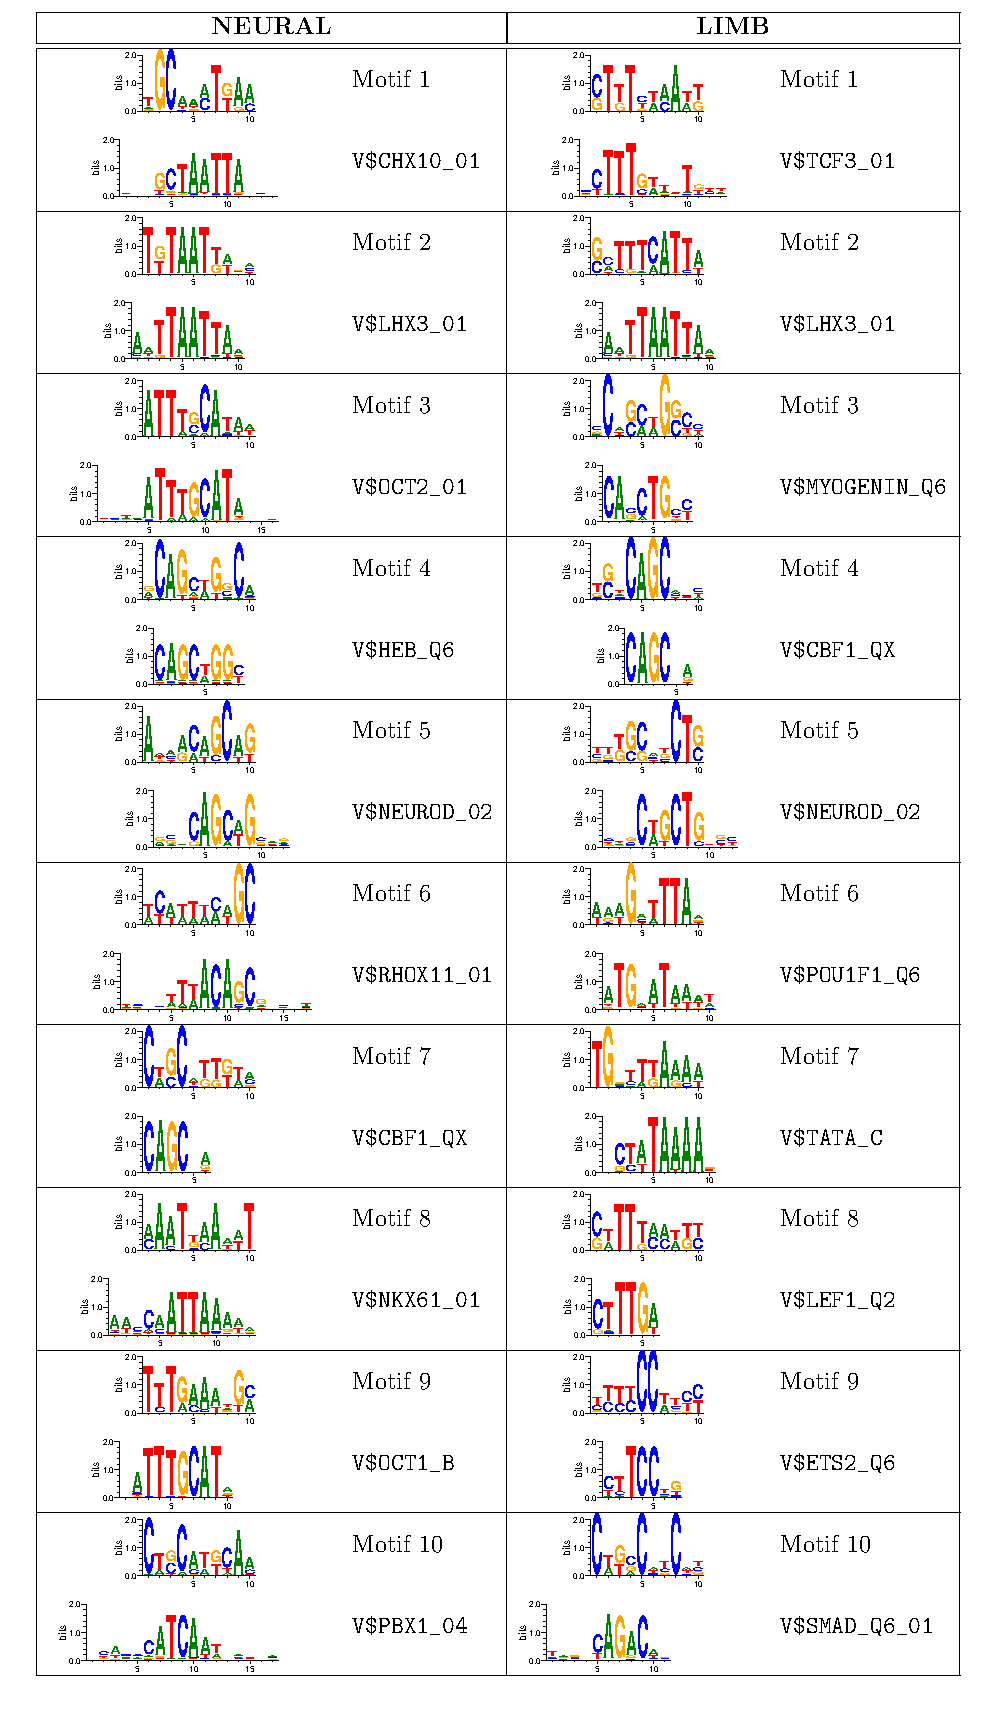
\includegraphics[height=20cm]{../figures-sub/figS2.pdf}
\end{center}
  \caption{ {\bf Motifs learnt on the full training sets.}
      The 10 best ranking motifs generated on the  CRMs training sets are
      shown together with the closest Transfac motifs (see {\em Distance between motifs} in {\em Methods} for details
     of motif distance computation).}
   \label{fig:motiftraining}
  \end{figure} 
   
    \begin{figure}[!htbp]
\begin{center}
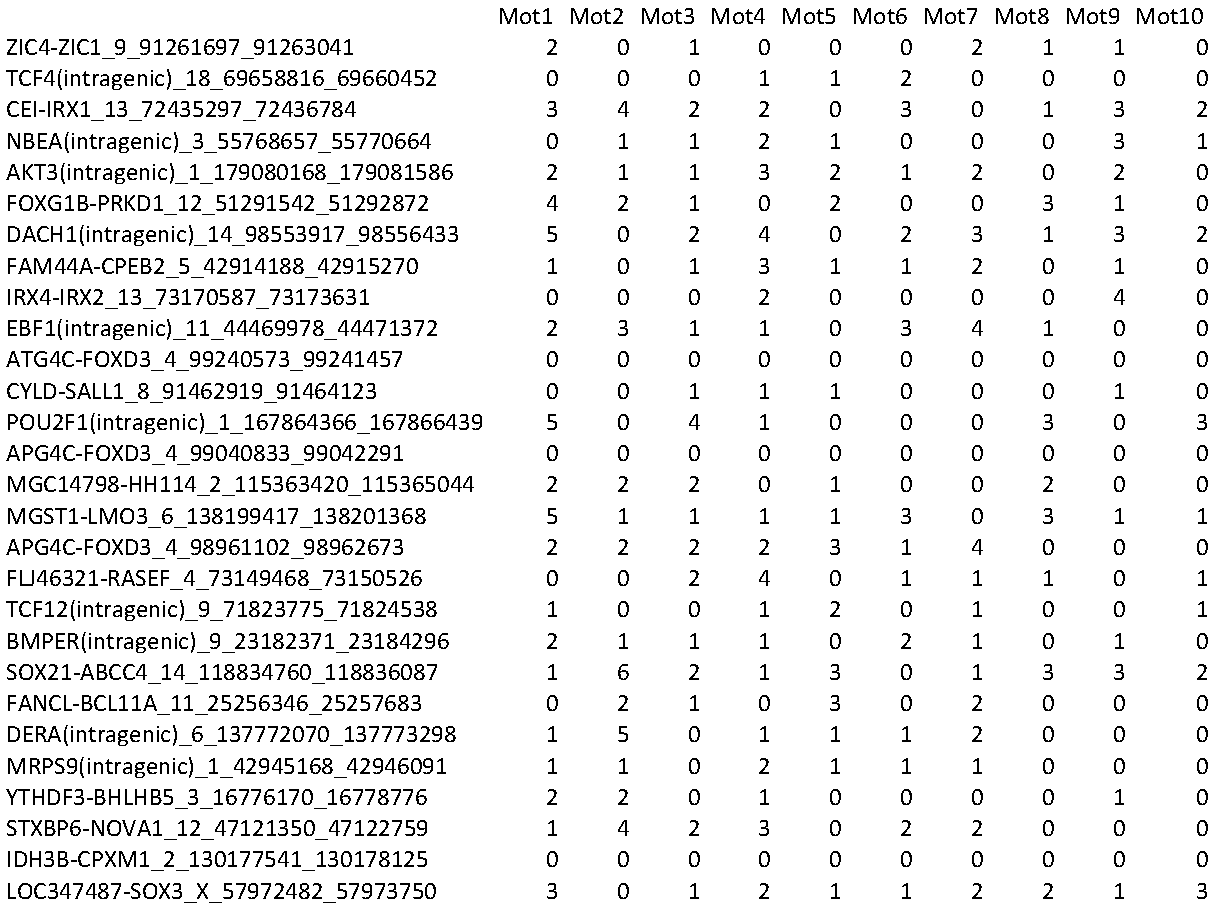
\includegraphics[width=17cm]{../figures-sub/figS3.pdf}
 \end{center}
\caption{{\bf Neural CRMs and motifs.}
    List of the neural CRMs used in this study.
The number of motifs of different types on each CRM is given for the 10
best-ranking neural motifs shown in Figure~\ref{fig:motiftraining}.}
\label{fig:ncrm}
\end{figure}

\begin{figure}[!htbp]
\begin{center}
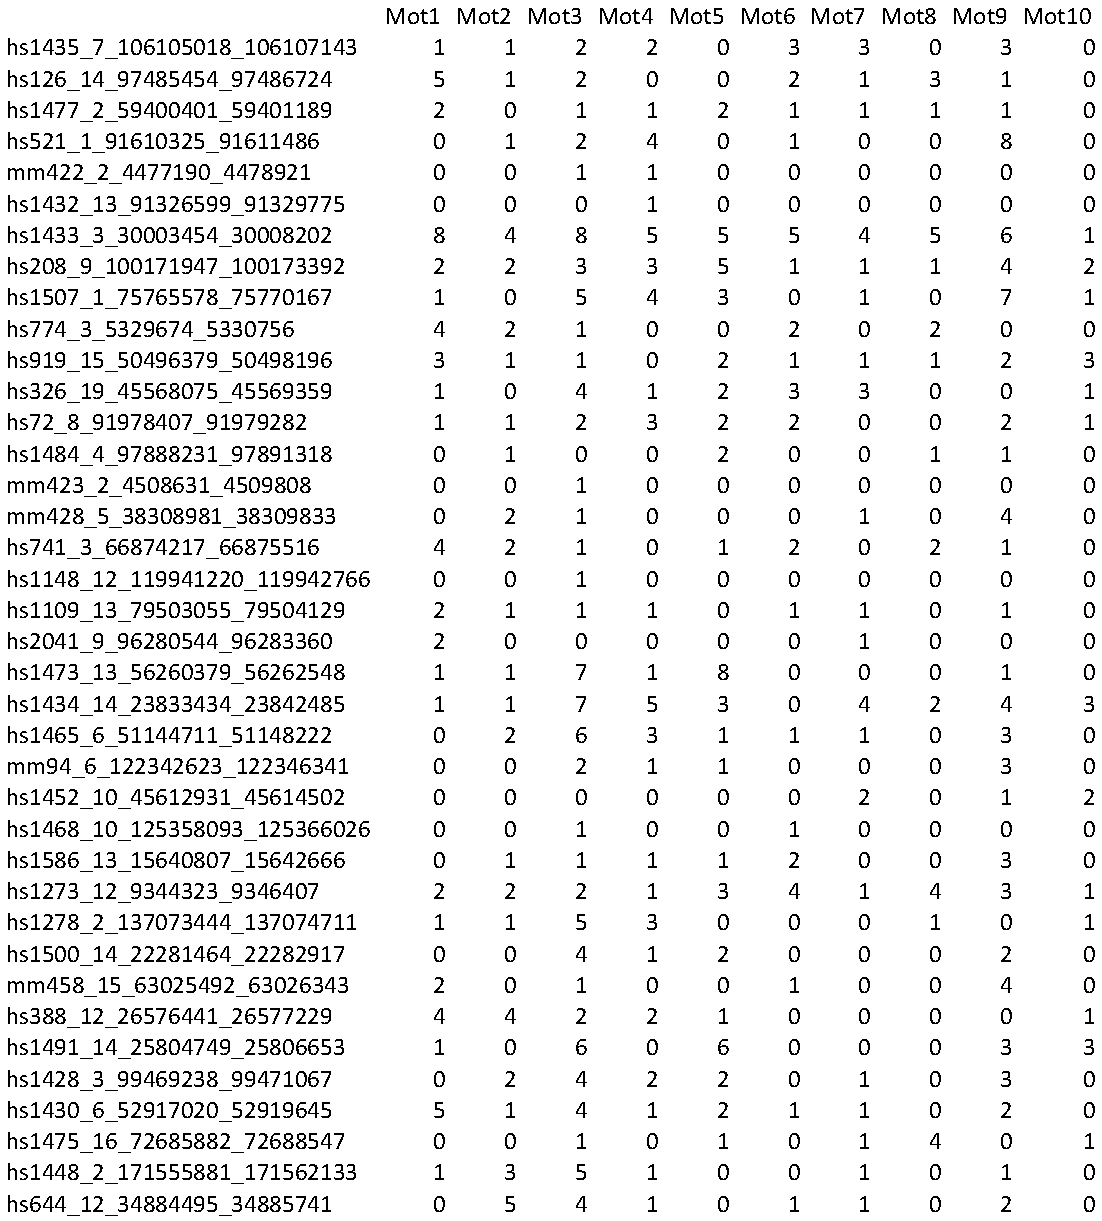
\includegraphics[width=17cm]{../figures-sub/figS4.pdf}
\end{center}
\caption{{ \bf Limb CRMs and motifs.}
List of the limb CRMs used in this study. The number of motifs of different
types on each CRM is given for the 10 best-ranking limb motifs shown in
Figure~\ref{fig:motiftraining}.}
\label{fig:lcrm}
\end{figure}

\begin{figure}[!htbp]
\begin{center}
   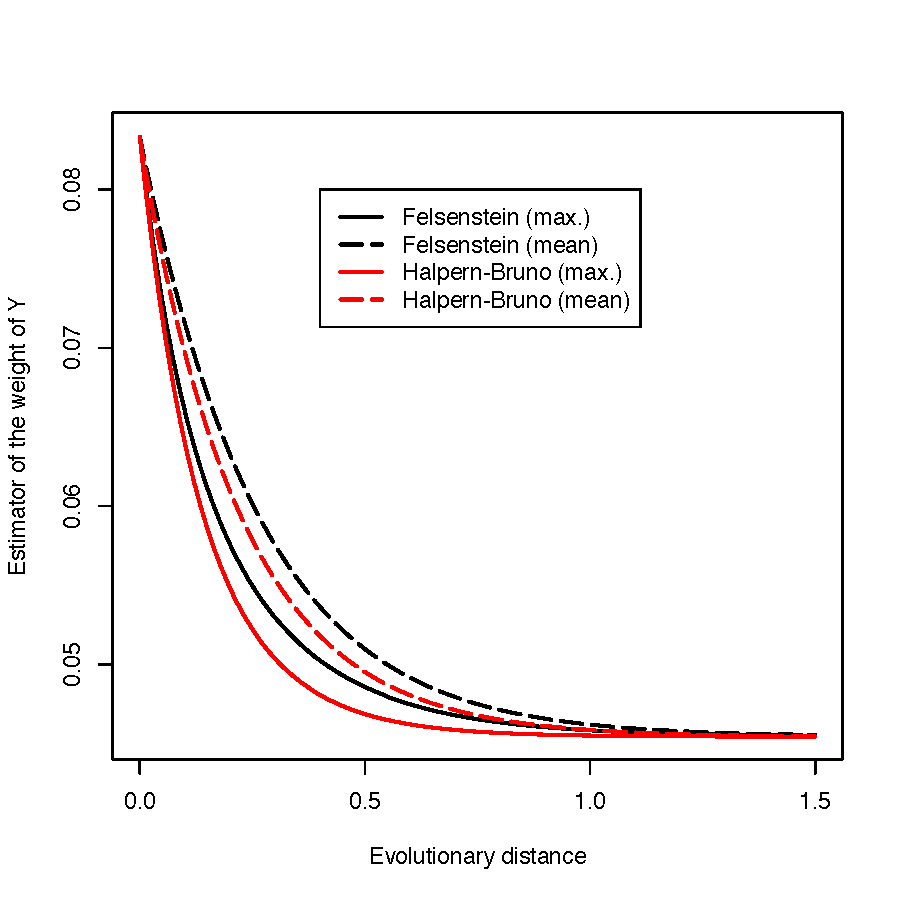
\includegraphics[width=10cm]{../figures-sub/figS5.pdf}
\end{center}
\caption{ 
{\bf  Simple example of motif inference with  Felsenstein and 
  Halpern-Bruno evolutionary models}  
    The inference of an ancestral base is compared in
    the simple case of two species at a phylogenic distance $d$
    from their common ancestor, for a two nucleotide alphabet,$X$ and $Y$.  
    The mean and maximum likelihood estimate of observing $Y$ in the 
    common ancestor given that the two species share an $X$ is shown as
    a function of evolutionary distance $d$, for the Felsenstein or 
    Halpern-Bruno evolutionary models.
    The likelihood is always smaller with the Halpern-Bruno model, reflecting
the model greater evolutionary rate.}
     \label{fig:evol}
    \end{figure} 


\bibliography{manuscript}


\end{document}



